%% print or electronic
\documentclass[ms,electronic,double]{nuthesis}

%% Needed to typset the math in this sample
\usepackage{amsmath}
\usepackage{amsfonts}
%% Let's use a different font
\usepackage[sc,osf]{mathpazo}

%% Makes things look better
\usepackage{microtype}

%% Makes things look better
\usepackage{booktabs}

%% Gives us extra list environments
\usepackage{paralist}

%% Be able to include graphicsx
\usepackage{graphicx}
%% Needed to display code 
\usepackage{listings}
\usepackage{algorithmic}
\usepackage{algorithm}
\usepackage{subfig}
\usepackage{url}
\usepackage{placeins}

%% I like darker colors
\usepackage{color}
\definecolor{dark-red}{rgb}{0.6,0,0}
\definecolor{dark-green}{rgb}{0,0.6,0}
\definecolor{dark-blue}{rgb}{0,0,0.6}
\definecolor{dark-purple}{rgb}{0.5,0,0.35} 
\definecolor{light-grey}{rgb}{0.9,0.9,0.9}

%% If you use hyperref, you need to load memhfixc *after* it.
%% See the memoir docs for details.
\usepackage[%
pdfauthor={Kartik Vedalaveni},
pdftitle={Adaptive Co-Scheduler for highly Dynamic Resources},
pdfsubject={Thesis},
pdfkeywords={LaTeX, Thesis, University of Nebraska, Intelligent Co-Scheduler},
linkcolor=dark-blue,
pagecolor=dark-green,
citecolor=dark-blue,
urlcolor=dark-red,
colorlinks=true,
backref,
plainpages=false,% This helps to fix the issue with hyperref with page numbering
pdfpagelabels% This helps to fix the issue with hyperref with page numbering
]{hyperref}

%Listings color code
\lstset{
language=c,
basicstyle=\ttfamily,
keywordstyle=\color{dark-purple}\bfseries,
stringstyle=\color{dark-red},
commentstyle=\color{dark-green},
morecomment=[s][\color{dark-blue}]{/**}{*/},
numbers=left,%left, right, none
numberstyle=\tiny\color{black},
stepnumber=1,
numbersep=10pt,
tabsize=4,
showspaces=false,
showstringspaces=false,
frame=single,
backgroundcolor=\color{light-grey}
}

%% Needed by memoir to fix things with hyperref
\usepackage{memhfixc}


\begin{document}
\frontmatter
\title{Adaptive Co-Scheduler for highly Dynamic Resources}
\author{Kartik Vedalaveni}
\adviser{Dr. David Swanson}
\adviserAbstract{Dr. David Swanson}
\major{Computer Science}
\degreemonth{August}
\degreeyear{2013}
\college{Graduate College}
\university{University Of Nebraska}
\city{Lincoln}
\state{Nebraska}
\doctype{Thesis}
\degree{Master Of Science}
\degreeabbreviation{M.S}
\maketitle

\begin{abstract}
 There are many kinds of scientific applications that are run on high throughput computational (HTC) 
grid. HTC may utilize clusters opportunistically, only running on a given cluster 
when it is otherwise idle. These widely dispersed HTC clusters are heterogeneous in terms of 
capability and availability, but can provide significant computing power in aggregate. The scientific 
algorithms run on them also vary greatly. Some scientific algorithms might use high rates of disk I/O 
and some might need large amounts of RAM. Most schedulers only consider cpu availability, but 
unchecked demand on these associated resources may give rise to several issues on the cluster.

On the grid there could be different schedulers on different sites and we cannot rely upon features 
of one kind of scheduler to characterize the nature and features of every job. Most state of the art 
schedulers do not take into account resources like RAM, Disk I/O or Network I/O. This is as true for the
 local schedulers as much it is for the grid. Often there is a need to extend these schedulers to solve 
 situations arising from new and/or complex use cases either by writing a plugin for existing schedulers or by Co­Scheduling. 
 A key issue is when resources like RAM, Disk I/O or Network I/O are used in an unchecked manner and 
 performance degrades as a result of it. Further scheduling jobs that claim the degraded resources could 
 overwhelm the resource to an extent that the resource will finally stop responding or the system will crash. 

With an increase in the number of entities concurrently using the resource, there is a
need to monitor and schedule concurrent and unmanaged access to any given resource to prevent
 degradation. These issues that we encounter in real life at the Holland Computing Center 
are the basis and motivation for tackling this problem and for developing an adaptive approach for scheduling. 
This co-scheduler must be aware of multi­-resource degradation, balance load across multiple sites and 
run clusters at high efficiency and share resources fluidly. An initial implementation in use at HCC will 
be evaluated and presented. 

  
\end{abstract}

%\begin{dedication}
%Dedicated to 
%\end{dedication}

\begin{acknowledgments}

First and foremost, I would like to thank my advisor Dr. David Swanson. Throughout my research
and writing he's been a constant source of support for me. His guidance and teachings have helped not 
only to shape my thesis but also in all walks of my life. I thank David for identifying this interesting
research problem and bringing it to me. His hard work has been constant source of inspiration.
 I'd like to thank Derek Weitzel for working with me to solve the 
 issues with grid submissions and for helping me with his technical expertise.
 
 I'd like to take this opportunity to thank the entire team at Holland 
Computing Center for providing me with the required resources, support and continuous advise
 even after I broke their systems. Its been a wonderful experience 
 working with these folks.
 
\end{acknowledgments}

\tableofcontents
\newpage
\listoffigures
\listoftables


%%   mainmatter is needed after the ToC, (LoF, and LoT) to set the
%%   page numbering correctly for the main body
\mainmatter

\chapter{Introduction}
Grid Computing as defined by Ian Foster in his paper The Anatomy Of the Grid \cite{Foster:2001:AGE:1080644.1080667}
states that 
\emph{Grid computing is about controlled sharing of resources with resource owners enforcing policies 
on the owned resources.} The resources come in the form of hardware 
and software that allows us to submit jobs, run the jobs and monitor the jobs on the grid. 
Universities usually have multiple clusters across their campus and these are 
usually owned by different departments but stand united under the banner of the university.
Campus grids can be thought of as mini grids in which jobs are spanned across multiple clusters
 based on the need of the user and available computing infrastructure within the computing resources across the university then often overflowed to the national
grid infrastructure\cite{derekThesis}.

Modern schedulers used in clusters provide numerable features for policy making, resource management 
and scheduling. The problem of cluster 
performance degradation that occurs when one of the resources is throttled is a problem that hasn't been 
addressed. The problem of performance degradation when many jobs are scheduled on a single system 
are either based on processor equivalence or based on the number of processor slots. Some of 
these schedulers like maui \cite{pbstorque} are sophisticated enough to take into account contention of other 
resources like RAM but ultimately convert the 2D vector values of CPU and RAM 
into a single scalar value which in-practice hard-codes the value or presents these resources
in a fixed ratio which makes us question effectiveness of such scheduling mechanisms. 

At Holland Computing Center present in University of Nebraska-Lincoln, we're 
tackling this issue of cluster degradation caused by 
over exploitation of one or more resources. 
The proposed solution adaptively schedules 
such highly dynamic resources on the grid and across multiple sites by adaptively scaling with respect to
the performance of a given cluster. We schedule based on minimum turnaround time of the sites which will help increase 
the throughput of the overall workload for the Co-Scheduler, which also is a good load-balancer in itself.

Existing schedulers depend on the availability of resources and frequent polling 
of it to determine the slots for scheduling. It should be noted that state of the art 
schedulers like maui/torque, slurm, condor take into account only CPU as a 
resource and the resources like RAM, Disk I/O or Network I/O are either ignored or 
their resource equivalent is converted into a scalar value which isn't an effective way of tackling the 
multiple resource scheduling problem .This might result in scheduling excessive jobs 
on single machine. In some schedulers, for example it'll be pre-assigned on every node that 1 CPU-CORE will have 2 GB of
memory. This kind of pre-assignment seems like it's addressing the resource degradation of RAM but suffers 
from the above mentioned problems.
We take a turnaround time approach to measure degradation, we define a resource 
to be degraded if and when we submit jobs that results in increasing the 
turnaround time by 25\% . It must be 
noted that there isn't explicit measurement of status of individual resources like RAM, Disk I/O, 
Network I/O. Since, there are no resource managers keeping track of these resource allocations. 
The Co-Scheduler is driven by the fact that turnaround time increases when 
concurrent jobs accessing these resources reach a threshold value which in-turn causes 
degradation and this is the basis for this work.

\begin{figure}[htbp!]
\begin{center}
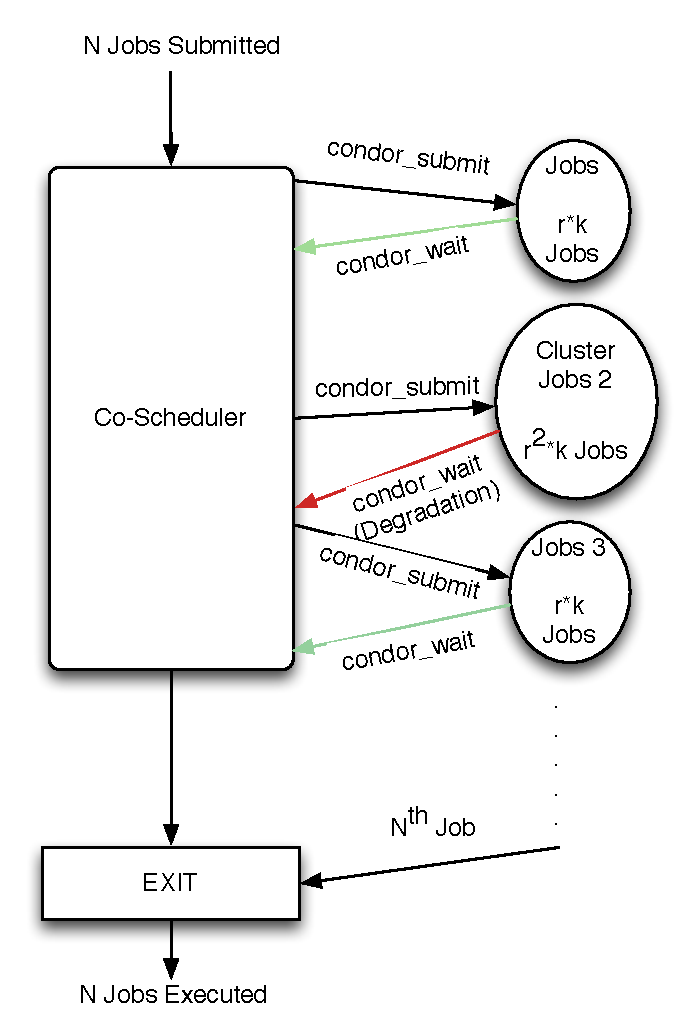
\includegraphics[scale=0.75]{images/degradation_detection}
\caption{Degradation occurrence: Co-Scheduling}
\label{fig:degradationdetect-intro}
\end{center}
\end{figure}

One aspect to Co-Scheduler is degradation detection and management by adapting 
to the throttling of a resource, another aspect is to efficiently distribute jobs 
across multiple sites which increases the throughput of the workload
. The Co-Scheduler adapts to degradation by backing off submission rates and waiting for a 
period of time (till the detection of optimal capacity) for the next incremental submission.It efficiently 
distributes the jobs and load-balances across multiple sites, thus submitting more 
jobs to a site with lesser turnaround time and also ensuring to submit lesser 
jobs to the sites with larger turnaround time. This efficiently load-balances 
across multiple sites on a grid and improves throughput because the loads may vary dynamically. 
The capacity of jobs the cluster can efficiently run without degradation needs to be detected and updated again and 
again after a given period of time.

In the figure \ref{fig:degradationdetect-intro}, with C1 called job propagation factor and k the initial number of 
jobs submitted we can see that on each iteration we're adding $k = C1 * k$ jobs, and on the
next iteration, if we have a degraded system, then we submit $k=k/C1$ amount of 
jobs by backing off on the amount of jobs submitted.

Finally, since the grid environment is a heterogeneous environment, it's absolutely necessary
to use APIs that are available on all the systems across the grid. To implement such a Co-Scheduler
 we limit ourselves to condor based clusters and utilize libcondorapi. The result is a threaded Co-Scheduler 
that submits to multiple sites concurrently and is aware of multiple-resource degradation and
loadbalances efficiently across multiple sites of the grid. 

Please note that all the references to the Co-Scheduler in this thesis refers to the adaptive Co-Scheduler designed 
by us.  

%% Thesis goes here
\chapter{Background}

\section{High-Throughput Computing} High Throughput Computing (HTC) is defined as 
a computing environment that delivers large amounts of computational
power over a long period of time.  The important factor being over a long period of time which 
differentiates HTC from HPC which focuses on getting large amount of work done in a small amount of time.
The workloads that run on condor systems don't have an objective of  how fast the job can be completed 
but how many times can the job be run in the next few months.In another definition of HTC, European Grid  
Infrastructure defines HTC as a computing paradigm that focuses on the efficient 
execution of a large number of loosely coupled tasks \cite{manual56}. One such 
distributed computing software providing High-Throughput Computing services is 
HTCondor developed by the condor team at University of Wisconsin-Madison.


\section{HTCondor} HTCondor is a distributed system developed by HTCondor team at the 
University of Wisconsin-Madison. It provides an HTC environment to sites 
that foster research computing and enables sites to share computing resources on otherwise  
idle computers at a given site. HTCondor includes a batch queuing 
system, scheduling policy, priority scheme, and resource classifications for a pool of 
computers, which is mainly used for compute-intensive jobs. HTCondor runs on both
 UNIX and Windows based workstations that are all connected by a network.  
Although there are other batch schedulers out there for dedicated machines. 
The power of condor comes from  the fact that  the amount of compute power 
represented by sum total of all the 
 non-dedicated desktop workstations sitting on people's desks is sometimes far 
 greater than the compute power of a dedicated central resource. There are many 
 unique tools and capabilities in HTCondor which make utilizing resources from 
 non-dedicated systems effective. These capabilities include process checkpoint 
 and migration, remote system calls and ClassAds. HTCondor also includes a 
 powerful resource manager with an efficient match-making mechanism that is 
 implemented via ClassAds, which makes HTCondor understandable when compared with other 
 compute schedulers\cite{manual56}. With numerous features of HTCondor, it is 
 used for grid computing on the scale of large number of massive computers 
 that are loosely coupled on the open science grid.
 
 
\section{Grid Computing}

As the cost of computers and the network connecting them is decreasing, there is movement towards a 
paradigm shift in computing with the clustering of geographically distributed 
resource. The goal of which is to provide a 
service oriented infrastructure  with organizations like the Grid community and Global Grid Forum 
constantly trying to invest effort in making Grid a platform with standard 
protocols, to provide seamless and secure discovery and access to infrastructure and interactions among
 the resources and services.
 
 With the advent of parallel programming and distributed systems it became 
 obvious that tightly coupled computers can be used for computing purpose and this 
 network of workstations  gave rise to the notion of distributed computing. 
 The Globus project began in 1996 and Argonne National Laboratory was responsible for a process 
 and middleware communication system called Nexus which provides remote service 
 requests across heterogeneous machines. The goal of Globus was to build a 
 global Nexus that would provide support for resource discovery, data access, 
 authentication and authorization.

At this point Grid replaced the use of metacomputer and \emph{ researchers from 
coolaboration of universities termed Grid as integrated resources 
with integration of many computational visualization and information resources 
into a coherent infrastructure.}

The following are goals and visions of Grid Computing:


\begin{description}
  \item[Seamless Aggregation of Resources and Services]
  Aggregation involves three aspects, 
  \begin{enumerate}
    \item{Aggregation of geographically distributed resources}
    \item{Aggregation of capacity}
    \item{Aggregation of capability}
      \end{enumerate}
    The key factors to enable such aggregation includes protocols and mechanisms 
    to secure discovery, access to and aggregation of resources for the 
    realization of virtual organization and applications that can exploit such 
    environment.

  \item[Ubiquitous Service-Oriented Architecture] This is the ability of the grid 
  environment to do secure and scalable resource and data discovery along with scheduling and 
  management based on a wide variety of application domains and styles of 
  computing.
  
  \item[Autonomic Behaviors]
  The dynamism, heterogeneity and complexity of the grid has made many 
  researchers rethink their systems. This new trend aims at system configuration 
  and maintenance of the grid with the least human effort and has led to numerous 
  projects like autonomic grids, cognitive grids and semantic grids.
  
\end{description}

At the heart of the grid computing tools provided by the open science grid lies globus toolkit, that provides
features and interfaces that enable grid computing. 
\section{Globus}
The Globus project is intended to accelerate the then meta-computing that build on 
distributed and parallel software technologies. The term meta-computing was used 
before the term grid was actually coined, refers to 
a networked virtual supercomputer, constructed dynamically from geographically 
distributed resources linked by high speed networks \cite{globus}. Scheduling 
and managing a large group of heterogeneous resources is a challenging and 
daunting task on the grid. The Globus toolkit provides a framework for managing 
and scheduling of grid resources across heterogeneous environments.

The Globus toolkit consists of a set of modules,  each module provides an 
interface for the provision of implementation of low level functionalities of 
the mechanisms of the toolkit:

\begin{itemize}
  \item{Resource location and allocation} 
  \item{Communications}
  \item{Unified resource information service}
  \item{Authentication interface}
  \item{Process creation}
  \item{Data Access}
\end{itemize}

There are multiple Virtual Organizations across Open Science Grid. One such VO 
is Nebraska's HCC VO at Holland Computing Center. A VO provides researchers with 
computing resources and enables sharing of resources across other VO's and 
additionally it signs the user's certificate so that a user is identified with a given VO.

We delegate our identification on the grid. \emph{voms-proxy-init}
is used to generate voms proxy at the submit host, we can specify voms as our 
virtual organization, hcc:/hcc in this case and hours as the number of hours the proxy would be 
active/valid, it must be ensured that the proxy period is approximately greater than the 
length of period of runtime of jobs for successful running of all the jobs. A 
proxy provides a secure way to access grid resources, by creating a proxy and 
delegating our identity to it for a short period of time enables us to sandbox 
the theft of the proxy credentials and limit the damage to the short lived proxy 
and keep our original set of credentials safe on the grid.

HTCondor-G extends condor to the grid environment, jobs are sent across grid universe using 
Globus software, Globus toolkit provides support for building grid systems but 
Submitting, managing and executing jobs have the same capabilities in both HTCondor 
and HTCondor-G world. Globus provides fault tolerant features to HTCondor-G 
jobs. GRAM is the Grid Resource Allocation and Management protocol, supports remote 
submission of computational request.

gt2 is an initial GRAM protocol which is used in Globus Toolkit version 1 and 
2. gt2 is also referred to as the pre-web services GRAM or GRAM2. Similarly, gt5 is the latest GRAM protocol, which is an extension of GRAM2 and is intended 
to be more scalable and robust, referred to as GRAM5.

\section{Open Science Grid} The Open Science Grid(OSG), provides service and support 
for resource providers and scientific institutions using a distributed fabric of 
high throughout computational services. OSG was created to facilitate data analysis from the 
Large Hadron Collider\cite{osg}. OSG doesn't own resources but provides software and services to 
users and enables opportunistic usage and sharing of resources among resource providers.
The main goal of OSG is to advance science through open distributed computing. 
The OSG provides a multi-disciplinary partnership to federate local, regional, community and 
national cyber-infrastructures to meet the needs of research and academic communities at all scales.

OSG provides resources and directions to Virtual Organizations(VO's) for the purposes of LHC experiments
and HTC in general. \\

Building an OSG site requires listing background and careful planning. The major 
components of an OSG site includes a Storage Element and Compute Element. \\
Storage elements (SE) manage physical systems, disk caches and hierarchical mass storage 
systems. A SE is an interface for grid jobs to underlying storage Storage Resource Management protocol (SRM) and Globus 
GridFTP protocol and others. A storage element requires an underlying storage system like hadoop, xrootd
and a GridFTP server and an SRM interface.\\
A Compute Element(CE) allows grid users to run jobs on your site. It provides a 
large number of services when run on the gatekeeper. The basic components include 
the GRAM and GridFTP on the same CE host to successfully enable file transfer 
mechanisms of Condor-G.\\


\chapter{Related Work}

\section{Comparison of existing mechanisms}
There are situations where we can have multiple condor pools exist and some of 
the pools have many idle slots that are available for utilization. To efficiently utilize the resources across pools condor provides 
mechanisms like condor flocking and condor job router. These mechanisms 
provide similar functionality to the Co-Scheduler designed here. In the following sections, we compare 
and evaluate these mechanisms with the design and functionality of Co-Scheduler.

\subsection{Condor Flocking}
Flocking refers to a mechanism where a job that cannot run on its own condor pool 
due to a lack of resources runs in another condor pool where resources are 
available. Condor flocking enables load sharing between pools of computers. As 
pointed out by Campus Grids Thesis\cite{derekThesis} flocking helps balance large workflows across different pools because of the scavenging and greedy nature 
of the condor scheduler.

To accomplish flocking Condor uses multiple components. 
\texttt{condor\_schedd} advertises that it has idle jobs to the remote \texttt{condor\_collector}. During the next phase of negotiation, if it's found that there are computers 
available then they are allotted to the jobs in the matchmaking phase and the 
jobs are then run on the remote pools. It so appears, and the local job queue's maintained as if 
the jobs are running locally. 

Although Condor flocking has workflow balancing features across multiple condor 
pools, it isn't aware of the slower and faster sites/pools. The adaptive Co-Scheduler 
keeps tabs on turnaround time and is aware of which site is faster or slower. If we 
look at the idea that scavenging idle resources increases throughput, it does. However If we look at the case where jobs are greater than the available slots 
across all the pools, condor flocking stops working here as deeper understanding of sites
would be required here to push more jobs at faster sites and importantly push less jobs
at slower sites, flocking's role is to scavenge idle computing slots across multiple pools. 

Another aspect where condor flocking isn't designed to perform well is when jobs are 
contending for the same resource (CPU, RAM, Disk I/O \& Network I/O). Even though we'll be 
having idle slot exist s on remote pools, condor flocking might not be able to use those 
slots as they'd be degraded because of the contention. In this case again 
Co-Scheduler comes in handy. Based on the turnaround time, Co-Scheduler waits for a random 
amount of time for degradation to clear and doesn't put excessive job load on the 
degraded resource. It diverts the jobs elsewhere to perhaps another site, which in-turn increases the 
throughput.

To conclude, we can say that condor flocking provides features of balancing 
large workflows and doesn't include features that would detect degradation in 
the cluster and also doesn't keep track of information of site performance, which might be exploited to increase the overall throughput of the system. 

\subsection{Condor Job Router}

The HTCondor manual defines the functions of job router to be the following:
\begin{quotation}

The Condor Job Router is an add-on to the \texttt{condor\_schedd} that transforms jobs from one type into 
another according to a configurable policy\cite{manual56}. 
This process of transforming the jobs is called job routing.
\end{quotation}

HTCondor Job Router can transform vanilla universe jobs to grid universe jobs and 
as it submits to multiple sites, the rate at which it starts submitting equals 
the rate at which the sites execute them. This provides a platform to balance large 
workflows across multiple grid sites and replenish the jobs at
faster sites once they get done. Job router sends more jobs to a site if 
the jobs submitted are not idle and stops submitting jobs if the submitted jobs 
sit idle on the remote cluster. Job router is not aware about which site is 
faster of slower.


\begin{figure}[htbp!]
\begin{center}
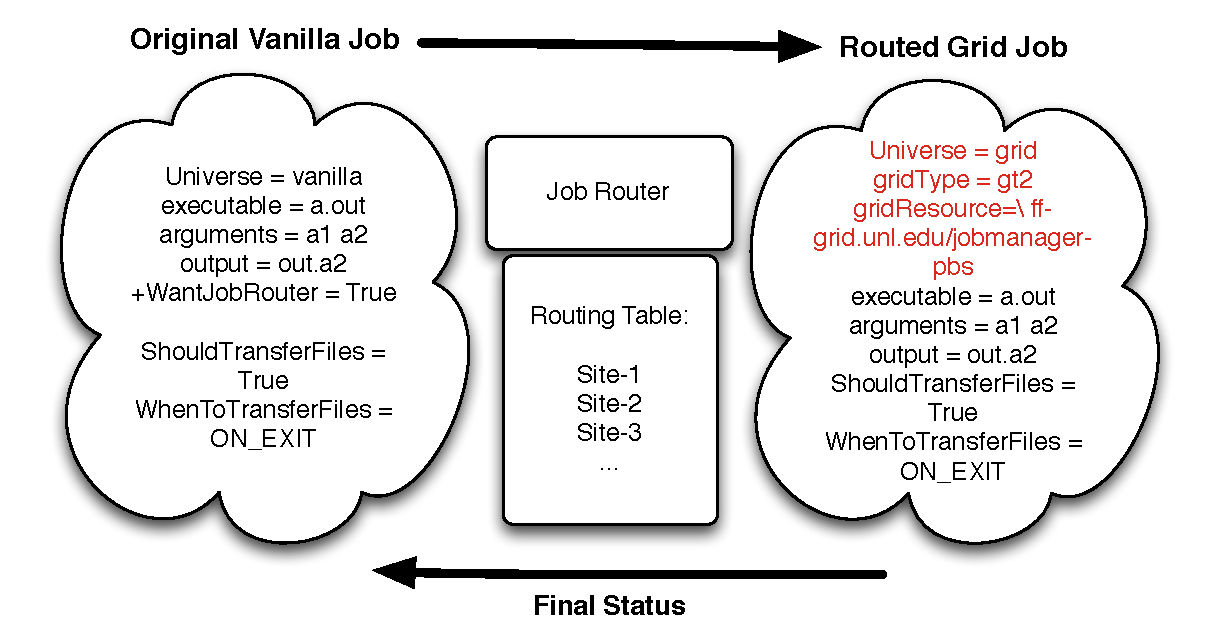
\includegraphics[scale=0.75]{images/jobRouter}
\caption{JobRouter: Transformation of Jobs}
\label{fig:JobRouter}
\end{center}
\end{figure}

A job is transformed to the grid universe by making a copy of the original job 
ClassAd and modifying some attributes of the job. This copy is called the routed 
copy and this routed copy shows up in the job queue with a new job id\cite{manual56}.

Condor job router utilizes a routing table which contains the listing of sites 
the job must be submitted to and the name of the potential grid resources, Routing is processed via a  condor config file which is defined by the new ClassAds.

\begin{figure}
\begin{lstlisting}
  # Now we define each of the routes to send jobs on
JOB_ROUTER_ENTRIES = \
   [ GridResource = "gt5 ff-grid.unl.edu/jobmanager-pbs"; \
     name = "Firefly"; \
   ] \
   [ GridResource = "gt5 tusker-gw1.unl.edu/jobmanager-pbs"; \
     name = "Tusker"; \
   ] \
   [ GridResource = "gt5 pf-grid.unl.edu/jobmanager-condor"; \
     name = "Prairiefire"; \
   ]\

\end{lstlisting}
\caption{Configuration to implement Job Routing}
\end{figure}

Condor Job Router appears to be a step up from the Condor Flocking in terms of 
scavenging resources and sending the extra jobs to another condor pool. Condor 
Job Router also maintains the submission rate of the jobs on submit hosts equal to that of remote clusters. But the job 
router does not keep track of how fast each condor cluster is. Thus 
condor job router does not optimize the displacement of jobs from a slower 
cluster. Since it maintains the rate of submission of jobs, we can be sure that if a job is completed 
at a faster site, it's immediately replaced by the next one. The same is true for a job at slower site 
too.
This might result in increasing the degradation if there exists some. For example, if the job router kept track of slower sites, it
can send less jobs to slower sites and thereby increase the overall throughput of the given workflow.

A preliminary examination shows that condor job router does seem to have degradation detection features, 
it does not submit to a pool that already has idle jobs however close examination reveals that even though it
submits to a pool with non-idle jobs it isn't aware of the fact that the jobs in the queue would have 
undergone degradation due to contention on same resource and thus isn't a viable mechanism for degradation detection.

\subsection{OSG Match Maker}

OSG Match maker is a tool that was created to be distributed among small to 
medium sized VOs to be used as a powerful submit interface to OSG. It is 
designed to retrieve VO specific site information and also to verify and 
maintain the sites by regularly submitting verification jobs to make sure site 
can continue receiving jobs.
OSG Match maker is another tool that provides information about the grid sites to the 
Condor scheduler. Condor scheduler does all the matchmaking with the classads attributes. 
  

\chapter{Adaptive Co-Scheduler For Highly Dynamic Resources}

\section{Introduction}
Due to the heterogeneous nature of the grid there could be problems with resource sharing on the grid. We propose a solution that primarily solves the problem of degradation due to contention among 
jobs for any given resource like RAM, I/O and the network. The contention among jobs sometimes give rise to 
degradation depending upon the availability of the resource that results in reduced performance of the cluster or crashes the cluster
altogether. Efficient and high throughput
distribution of jobs across multiple cluster is another challenging problem that we have solved in 
this particular Co-Scheduler Solution. 

\section{Degradation detection and Capacity based scheduling}
In the first part of the solution we target the basic problem of degradation. To give an example, suppose
we have a file server that can serve 100 MBps of data which is available for concurrent access and a user has submitted 200 jobs
each consuming 10 MBps of data I/O. If 100 CPU slots are available, a typical state of the art Scheduler
schedules these 200 jobs without actually looking at the I/O load. This results in a degraded system, 
over time if more jobs are Scheduled to utilize this file server. This file serve might even crash. We would need a 
degradation handling mechanism that would adaptively scale with the load and  exponentially 
back off during a high contention period. Thus we need an intervention in the form
of a Co-Scheduler that intelligently handles degradation. 
We start the capacity algorithm by submitting jobs to the cluster and measure 
the turnaround time of each iteration. If we find that the current turnaround 
time of an iteration is 25\% greater than the previous iteration we term it as a 
degradation. We now try to find the best capacity of jobs between the current 
and the previous iteration by exponentially backing off between these two iteration. We keep finding the optimal
capacity dynamically for each iteration as the contention may change and optimal capacity keeps 
 varying. Once the optimal capacity is found then it is retained for job submissions for a given amount of time
 limited to a maximum of ten iterations of jobs, thus solving the problem of performance degradation. 

\section{Multi-site load distribution based scheduling} 
 \begin{figure}[htbp!]
   
 \begin{verbatim}
 C1 -> Job propagation constant
 multiSite -> list storing turnaround times of multiple sites.
 low ->  min(multiSite)  
 high -> max(multiSite)
 avg -> average(multiSite)
 \end{verbatim}

$$
f(C1) = \left\{
        \begin{array}{ll}
            C1*4 & \quad multiSite_i = low\\ 
            C1/2 & \quad multiSite_i = high \\
            C1*2 & \quad multiSite < avg
        \end{array}
    \right.
$$

\caption{Multi-site Job distribution function}
  \label{fig:multiSite2}

\end{figure}
Since we're already tracking site performance, the other problem that we tackled was that of efficient distribution of work load to multiple sites of the 
grid, refer to the \ref{fig:multiSite2}.
Some of these sites could be error prone, some of them could be faster and some can be slower. We need to
take an approach that improves the overall throughput of the workload, thus we keep track of average turnaround
 time for each batch of jobs submitted to the cluster. We take the average turnaround time of the batch of jobs that is submitted 
 across multiple clusters. We group turnaround times of these batches of jobs based on the value of the 
 turnaround time to be greater than, less than, or equal to the average turnaround time of all batch of jobs.
 This gives us a classification of sites that run faster, we exploit this information in our scheduler. 
 To implement multi-site job submission and load balancing we start submitting one job to each cluster 
 and measure the turnaround time once the job returns. Now we have the information of turnaround time 
 of a particular resource of all the clusters. Continuing to submit jobs concurrently in a similar manner
  would result in the completion of
 the workload in a non efficient way. Out of the list of all the turnaround times of different sites we take the 
 sites
 that have lower than average turnaround time of all batches of jobs and increase the job propagation 
 factor for these jobs. This in-turn increases the number of jobs submitted to that site and helps us efficiently distribute 
 the workload to faster clusters ( submitting to a faster site would enable us to submit 
 more jobs to the particular site. As the turnaround time is lower we would finish jobs quickly and make room for more
 jobs if we submit less to slower sites. These sites can still help us improve the throughput to a greater extent by enabling us to 
 prevent further degradation at those sites.
  ) 
  Error handling mechanism is gracefully handled by 
 condor and by this approach we have an efficient system with increased throughput and with proper distribution
  of load across multiple clusters.  
        
 
 
 
%%A table of comparison among all three kinds of mechanisms


%\chapter{Design and Implementation of Co-Scheduler}
%(an image to showcase layer of position of co-scheduler)
The co-scheduler requires the presence of a condor installation and libcondorapi.
It is written in the C++ language and has extensively made use of pthreads for 
synchronization and multithreading. The co-scheduler has two components to it,the first one is a capacity detection
algorithm which is found by measuring degradation and the other aspect to it is 
multi-site workload distribution algorithm .The following paragraphs detail the 
engineering aspects of the design.
The program begins by taking the number of jobs, site's information and submit script 
information as its input. The number of jobs are the ones submitted across 
multiple sites. The next input file contains information on the list of sites that can be used 
for load balancing in the GridResource format of the condor ClassAds API, e.g. \emph{tusker-gw1.unl.edu/jobmanager-pbs}.
It is assumed that all the sites listed in the sites input file are working and 
do not have any misconfiguration issues. The third and the final option to the 
scheduler is the submit description file. All the job ClassAd information and 
requirements can be written in this section and all of these will be applicable on the grid when a particular job is 
scheduled. The two main important attributes required in the submit description 
file is \emph{universe} which needs to be grid all the time as we are submitting 
to grid sites, and the other most important thing is the 
\emph{grid-proxy}. 
As we know that \texttt{condor\_wait} \cite{manual56}can be used to wait for a certain job or 
number of jobs to complete, it watches the log file and sees if the completion 
entry of the job is made in the log file that is generated by the \emph{log} 
command in the condor submit description file. There are two options we can 
specify to \texttt{condor\_wait} one is \texttt{-num}, \texttt{number-of-jobs} that waits
till the \texttt{number-of-jobs} are completed and the other option is to specify \texttt{wait}, seconds that 
waits for seconds amount of time. If nothing is specified \texttt{condor\_wait} waits indefinitely till
the job(s) are complete.

\section{Implementation of Capacity based scheduling}

This algorithm detects degradation and once we detect degradation we find the 
optimal capacity:

\begin{algorithm}
\begin{algorithmic}
\STATE $c2 \gets 1.25$ 
\COMMENT {c2: Degradation factor}
\WHILE{true}

\IF{T2 $<$ c2*T1}
  \STATE $jobSubmission(k)$ 
  \COMMENT {Submit k jobs}
  \STATE $T1=(T1+T2)/2$
\ENDIF

\IF{T2 $>$ c2*T1}
  \STATE $degradation\_high \gets k$
  \STATE $degradation\_low \gets k/2$
  \STATE $optimalCapacity(degradation\_high,degradation\_low)$
\ENDIF

\ENDWHILE

\end{algorithmic}
\caption{Algorithm for determining optimal capacity by detecting degradation}
\label{alg:Degradation Detection}
\end{algorithm}


\begin{algorithm}
\begin{algorithmic}

\STATE $mid \gets (high+low)/2$ 
\STATE $k \gets mid$
\STATE $jobSubmission(k)$ 
  \COMMENT {Submit k jobs}
\IF{T2 $<$ c2 * T1}
\STATE $T1 \gets (T1+T2)/2$
\STATE optimalCapacity(mid,high);
\ENDIF  
\IF{T2 $>$ c2 * T1}
\STATE optimalCapacity(low,mid);
\ENDIF
\RETURN mid
\end{algorithmic}
\caption{Algorithm for determining optimal capacity by detecting degradation}
\label{alg:optimalCapacity(high,low)}
\end{algorithm}

Algorithm \ref{alg:Degradation Detection} sets up the stage for degradation 
detection, it submits more jobs if the T2 is within permissible limits else the 
algorithm calls the optimal capacity algorithm that detects optimal capactiy.

Algorithm \ref{alg:optimalCapacity(high,low)} is passed two parameters high and 
low. These represent the upper bound where degradation has taken place and lower bound 
where degradation hasn't taken place. The algorithm works like a modified binary 
search and takes O(log n) iterations to find the optimal set of jobs.

\section{Implementation of Multi-site load distribution based scheduling}
In figure \ref{fig:multiSite1}. Multi-site load distribution based scheduling uses the turnaround time at each 
site for sending future jobs, its a threaded algorithm, the following is extracted function per thread:

\begin{algorithm}
\begin{algorithmic}

\STATE $c1 \gets 2$ 
\COMMENT {c1: Job propagation factor}
\COMMENT {multiSite is a list storing turnaround times of multiple sites.}
\STATE $low = min(multiSite)$
\STATE $high = max(multiSite)$
\STATE average = $\sum_i multiSite_i$ / Sizeof($multiSite_i$)

\IF{turnaroundTime\_Thread $==$ low}
\STATE $c1 \gets c1 * 4$
\ENDIF

\IF{turnaroundTime\_Thread $==$ high}
\STATE $c1 \gets c1/2>1 ? (c1/2:1)$
\ENDIF

\IF{turnaroundTime\_Thread $<$ average}
\STATE $c1 \gets c1 * 2$
\ENDIF

\end{algorithmic}
\caption{Algorithm for distribution of workflow load across multiple sites on the grid}
\label{alg:updateJobPropagationConstant()}
\end{algorithm}

Algorithm \ref{alg:updateJobPropagationConstant()} classifies different sites 
into faster and slower sites based on the performance of the sites bound by the 
turnaround time for the purpose of multi-site load distribution algorithm.

\begin{figure}[htbp!]
\begin{center}
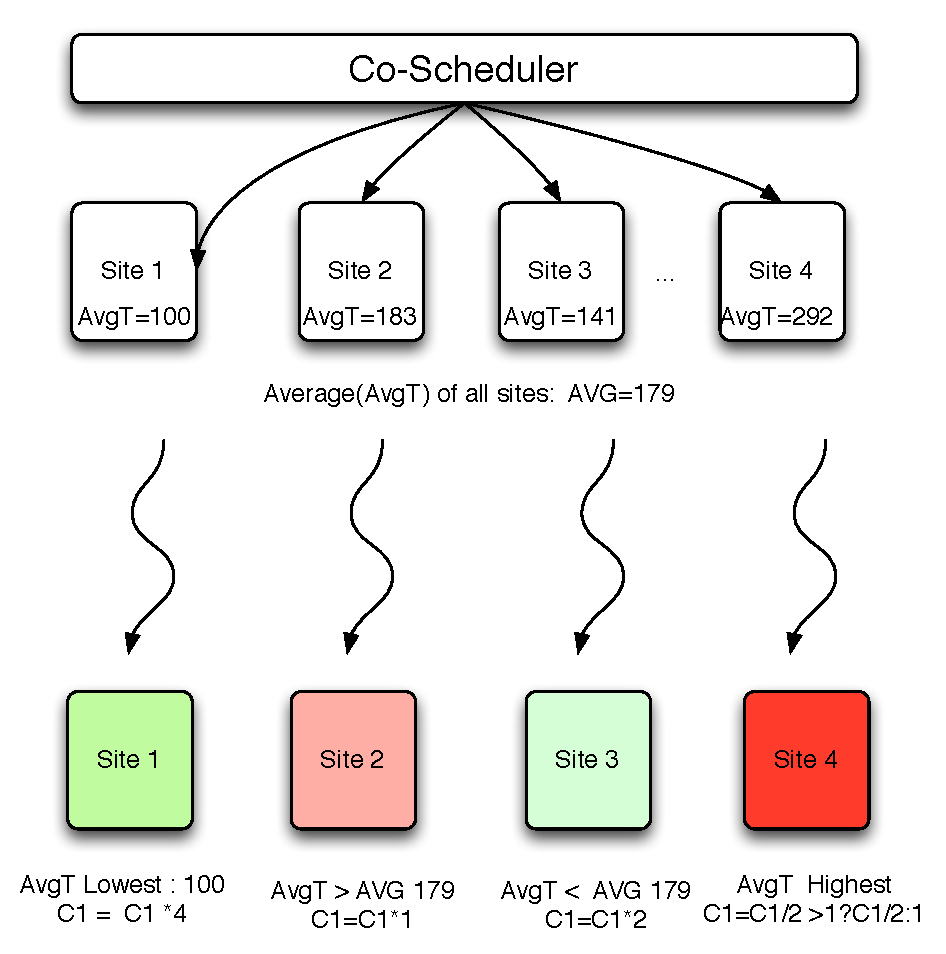
\includegraphics[scale=0.75]{images/multipleSites}
\caption{Multi-site scheduling algorithm overview, classification of sites into slower and faster}
\label{fig:multiSite1}
\end{center}
\end{figure}
\FloatBarrier
Diagram:
\section{Programming APIs}
\subsection{HTCondor Log Reader and User API}

HTCondor provides Job Log Reader API\cite{manual56} that polls logs for job events by giving us 
API access to the events and outcomes. The following is the constructor for 
initializing a ReadUserLog object.

Constructor:
ReadUserLog reader(fp,false,false);
\begin{verbatim}
ULogEventOutcome (defined in condor_event.h):

Status events for job detection:

ULOG_OK: Event is valid
ULOG_NO_EVENT: No event occurred (like EOF)
ULOG_RD_ERROR: Error reading log file
ULOG_MISSED_EVENT: Missed event
ULOG_UNK_ERROR: Unknown Error
\end{verbatim}

All the entries in the log file end with \texttt{...}. All the job 
log entries are named as events and these events could range from being  \texttt{ULOG\_OK} where 
the event has taken place and is valid to \texttt{ULOG\_UNK\_ERROR} where an error has 
taken place.

The following pseudo-code is extracted from the logReader module that first 
detects all the valid events and then based on the data-structure of the event 
object detects if the event kind is \texttt{ULOG\_EXECUTE}, meaning the job has begun 
executing, via eventNumber data member. Finally, we detect the \texttt{ULOG\_JOB\_TERMINATED} 
event where the job has successfully terminated. We also cast the more general event 
object into JobTerminatedEvent to access data members of the 
JobTerminatedEvent. The comments in the listed pseudo-code provides more details 
on this extracted code.


Job Submission Pseudo-Code:

\begin{lstlisting}
void logReader(string hostFile, args *data, int nSites)	{		
		FILE *fp;
		ReadUserLog reader(fp,false,false);
		ULogEvent *event = NULL;		
             while(reader.readEvent(event)==ULOG_OK)	{                    
            if((*event).eventNumber==ULOG_EXECUTE )	{                                
            //Cast into Execute Event
                ExecuteEvent *exec 
                = static_cast<ExecuteEvent*>(event);                                       
                //condor_wait -num K, where K is the 
                //amount of jobs completed till the wait.
                    char tmp[100];
                    sprintf(tmp,"condor_wait -num 
                    \%d \%s",count,hostFile.c_str());
            }            
            if((*event).eventNumber==ULOG_JOB_TERMINATED)	{                
            //Cast into Job Terminated Event
                JobTerminatedEvent *term 
                = static_cast<JobTerminatedEvent*>(event);                
                
                if(term->normal)	{                    
                    //on Normal termination, 
                    //works only for local jobs, 
                    //find the CPU time of local jobs
                }               
            }
        }
}

\end{lstlisting}
\subsection{Synchronization Co-Scheduler Code}

There are critical sections in the code where synchronization becomes absolutely 
necessary. One such variable is number-of-jobs. The number of jobs executed across 
the sites should remain fixed and the value must match the value that has been 
given as input. In a threaded system where each thread is executing jobs on a 
different cluster it becomes necessary to define \texttt{N}, the number of jobs executed or executing as a 
critical section. Here we define a pthread mutex and lock it for all write accesses to the \texttt{N}
, we serialize the access to \texttt{N} and make conditional checks during job submission, so as not to allow
job submissions when \texttt{N} is greater than the input value. By 
serializing the access across multiple threads the total jobs executed remains 
equal to the input number of jobs. The following chunk of code block 
demonstrates the use of mutexes for serialization of  \texttt{N} among the threads.

\begin{figure}[htbp!]

\begin{lstlisting}
pthread_mutex_t mymutex = PTHREAD_MUTEX_INITIALIZER;
pthread_mutex_lock (&mymutex);
sumOfK+=k;
pthread_mutex_unlock (&mymutex);
\end{lstlisting}

\caption{Mutex on Number Of Jobs, sumOfK variable}
\label{fig:mutex}

\end{figure}


Another section of code where synchronization becomes important is while 
distributing the jobs to multiple sites. When measuring which cluster is 
faster, we need information of turnaround time from all the sites 
before proceeding, this means all the threads need to be executing the same line of code 
before proceeding with the further program. Thus the absolute need for 
synchronization. To handle this problem we make use of conditional pthread variable. The following code demonstrates the use of conditional wait 
and conditional signal variable that clears the block on all the threads waiting 
based on the given condition.


\begin{figure}[htbp!]

\begin{lstlisting}
pthread_mutex_t syncMutex = PTHREAD_MUTEX_INITIALIZER;
pthread_cond_t synchronize_cv = PTHREAD_COND_INITIALIZER;

pthread_mutex_lock(&syncMutex);    
multiSite.push_back(stats[thread_id].T1);	
tid_multiSite.insert(std::pair<int,int>
(data->tid,stats[thread_id].T1)
);
	   
if ( multiSite.size() < numOfSites )
{
  pthread_cond_wait(&synchronize_cv, &syncMutex);
}
else
{		
pthread_cond_broadcast(&synchronize_cv);
}
pthread_mutex_unlock(&syncMutex);
    
\end{lstlisting}
\caption{Synchronization of threads after reading turnaround time}
\label{fig:synchronization}
\end{figure}
\FloatBarrier

We need to have the turnaround time of the first job,  which enables us to measure 
how fast each cluster is. To do so, we need to wait for each job to complete on 
the first submission thereafter the jobs are submitted asynchronously and the 
average turnaround time is updated in the list. In this pseudocode the threads 
beginning first add the turnaround time to the list and conditionally wait if 
the size of the list is less than the number of sites. The last thread comes in 
and the same condition is voided and executes a conditional broadcast to unblock 
all the waiting threads and the scheduling proceeds further to asynchronously schedule further 
jobs.
In this example of synchronization code there is a possibility that some of the 
threads wait continuously if the availability of the sites is very low. 
Currently we assume the existing availability of the cluster for the above code 
to take effect and reserve the function of deadlock prevention of some threads 
dude to bad sites for future work.

\chapter{Evaluation}

We evaluate the degradation detection algorithm by the distribution of turnaround time. The turnaround 
time of all the jobs when run using co-scheduler and the turnaround time of all 
the jobs when run directly on the cluster using the condor-g grid interface were both investigated.

If a NFS server has the capacity to serve 50 clients without degradation it
implies the turnaround time of all the jobs on the 50 clients are within the 
limits that would not be a degraded turnaround time. If the same NFS server is forced to serve 200 
clients then we would see a degradation and would see an increase in the turnaround time of the jobs
that are now contending for the I/O. This would result in degraded turnaround time and 
the same jobs would have to take lot more time to complete which is the usual 
scenario that occurs at Holland Computing Center when large amount of I/O bound 
jobs are submitted to the cluster and there is no check on the usage and the 
capacity of the I/O resource.

In this evaluation, we've submitted 375 jobs to a cluster tusker using bulk 
condor-g submission and then submitting it through the co-scheduler so that we 
can keep track of degradation, detect it and prevent it. The submit scripts for 
the co-scheduler are generated dynamically and the grid universes are populated 
from the input sites file. The machine that is used for jobs submission is a 
condor developmental virtual machine. That had to be configures for the grid 
submissions before its use for the experiment. 375 Jobs were run on the lustre 
filesystem and the results for this run in figure \ref{fig:tusker_histogram} is 
of the production level tusker. We were able to see degradation when we 
submitted jobs in bulk using condor-g interface but we couldn't be sure if the 
degradation was the result of just our I/O based test job. Thus separate 
individual NFS servers were setup on both the clusters sandhills and tusker and 
tests were run again. The results of the tests are projected in the figure \ref{fig:nfs_tusker_histogram} 
and figure \ref{fig:nfs_coscheduler_tusker_histogram}.

As stated above we're making use of histogram of binned turnaround time and good 
put graphs to study the effect of degradation. Ideally a histogram that projects 
degradation has many jobs that have higher turnaround times compared to a non 
degraded graph. A histogram that doesn't project degradation will have most of 
its jobs with the permissible limits of turnaround time and wouldn't have large 
variance in terms of the turnaround time. We also make use of goodput graphs 
that plot an area graph w.r.t the turnaround time. It provides a good way to 
visualize the turnaround time. Ideally the area under the curve must be minimum 
in case of a non degraded graph but in a graph that projects degradation the 
area under the curve is larger than its non-degraded counterpart.

Figure \ref{fig:tusker_histogram} shows how there exists a large variance in 
turnaround time by having a larger turnaround time than that present in figure 
\ref{fig:coscheduler_histogram}. The former was the result of bulk submission 
whereas the later is the result of co-scheduler run. The associated goodput 
graphs in figure \ref{fig:tusker_jobgoodput} and figure \ref{fig:coscheduler_jobgoodput} 
show thir respective areas with degraded run taking up larger area. When we look 
at the turnaround time distribution on independent NFS servers we can inter many 
things, that the degradation is lot significant in the figure \ref{fig:nfs_tusker_histogram} and the co-scheduler 
resolves degradation to a larger extent as noted in figure 
\ref{fig:nfs_coscheduler_tusker_histogram}.


\begin{figure}[h!]
\begin{center}
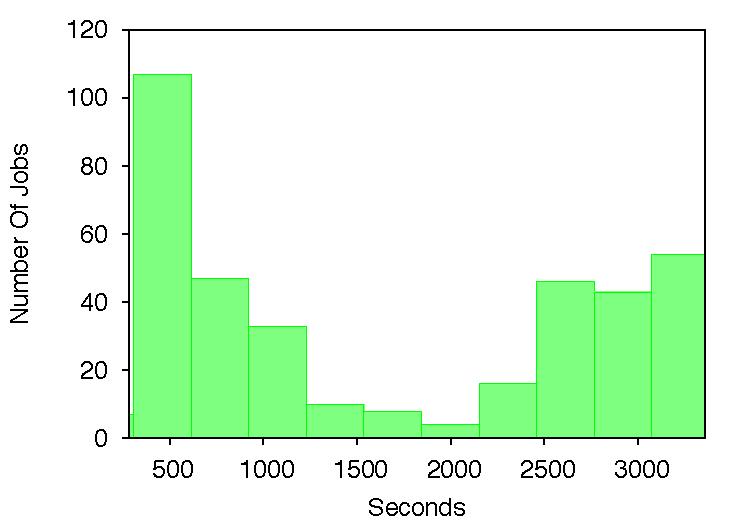
\includegraphics{images/tusker_histogram}
\caption{Histogram showing turnaround time distribution of 375 Jobs, when run on Tusker cluster}
\label{fig:tusker_histogram}
\end{center}

\begin{center}
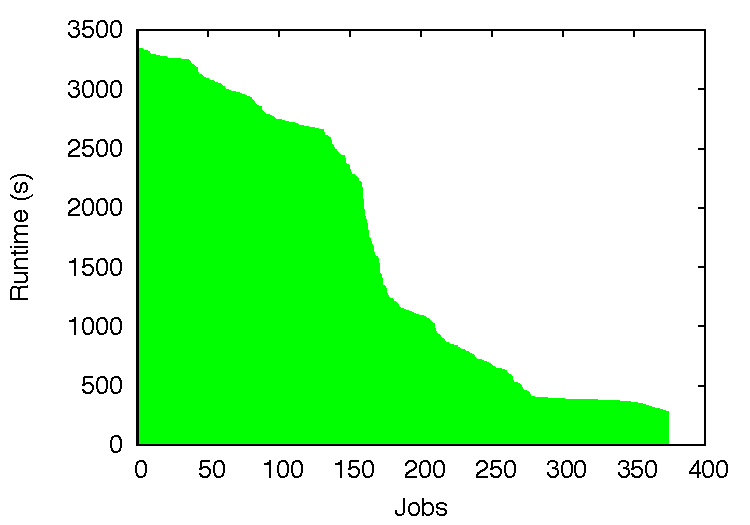
\includegraphics{images/tusker_jobgoodput}
\caption{Goodput graph showing the turnaround time distribution of all the jobs submitted}
\label{fig:tusker_jobgoodput}
\end{center}

\end{figure}
\FloatBarrier

The test I/O job used in this experiment continuously does disk write operations for a given period of time, the average
time taken by the program being 300-500 seconds when run on different resources and generated approximately 3 GB of data file
in that period. It was necessary to design our own test I/O program because of the need to change the path
to the NFS servers where we'd be doing our benchmark to test the servers. The test I/O job takes two parameters
one is the size N and the other is the path where the I/O must take place. There are two 
clusters under consideration, Sandhills and tusker. 375 jobs are run on each of 
the clusters and then a separate set of 375 jobs are scheduled using 
Co-Scheduler. We measure the extent of degradation on each cluster and quantitatively 
determine how degradation is handled by the Co-Scheduler.

In figure \ref{fig:tusker_histogram}  considerable jobs take more than 2500 seconds to complete. 
When the resource is not degraded the test Job takes approximately 300-500 seconds of time.Tusker is 
currently running Lustre filesystem. If the capacity of the filesystem permitted 
to serve 375 jobs(or the number of jobs running concurrently) then most jobs 
would be completed within 500 seconds of time but that isn't the case with the 
tusker and hence we can conclude the resultant graph is the cause of degradation 
of disk I/O resource but there needs to be clarification about the source of the degradation. 
It could either be caused by the test I/O jobs that were submitted or can be caused 
by a set of jobs that are already running on the cluster. To clarify this issue 
and get a clear picture on whats causing the degradation the result from the 
figure \ref{fig:nfs_tusker_histogram} sheds more information.


\begin{figure}[h!]
\begin{center}
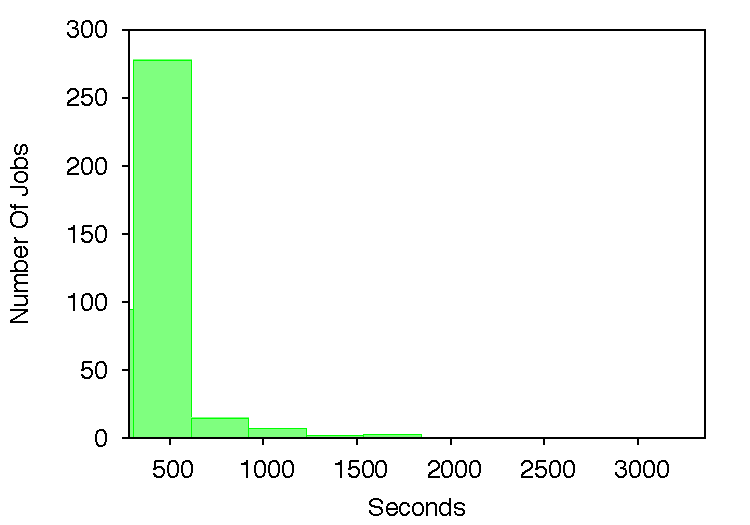
\includegraphics{images/coscheduler_histogram}
\caption{Histogram showing turnaround time distribution of 375 Jobs, when run on Tusker cluster}
\label{fig:coscheduler_histogram}
\end{center}

\begin{center}
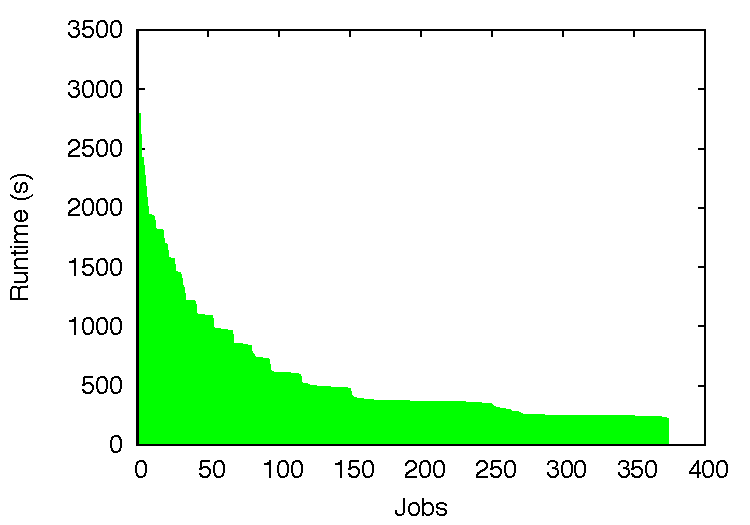
\includegraphics{images/coscheduler_jobgoodput}
\caption{Goodput graph showing the turnaround time distribution of all the jobs submitted}
\label{fig:coscheduler_jobgoodput}
\end{center}

\end{figure}
\FloatBarrier

\begin{figure}[htbp!]
\begin{center}
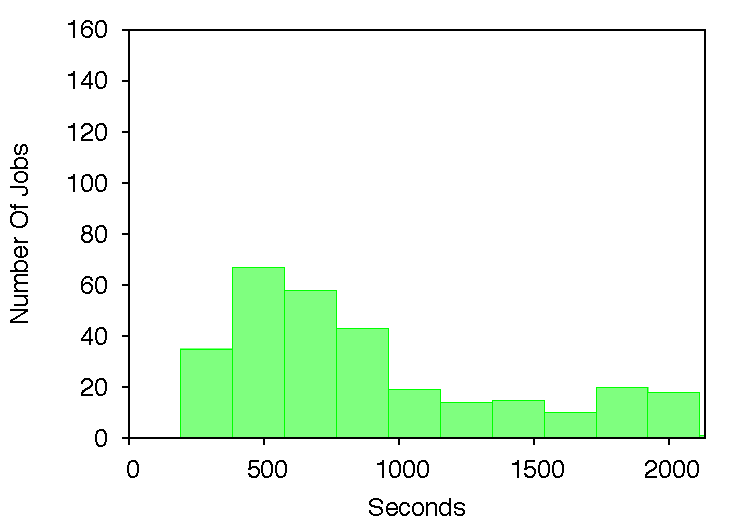
\includegraphics{images/nfs_tusker_histogram}
\caption{Histogram showing turnaround time distribution of 300 Jobs, when run using a coscheduler on a custom small scale independent NFS server}
\label{fig:nfs_tusker_histogram}
\end{center}

\begin{center}
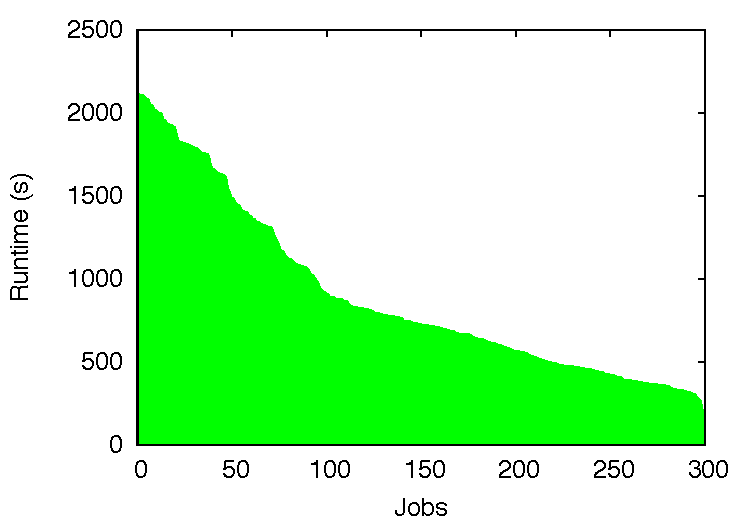
\includegraphics{images/nfs_tusker_goodput}
\caption{Goodput graph showing the turnaround time distribution of all the jobs submitted}
\label{fig:nfs_tusker_goodput}
\end{center}


\end{figure}
\FloatBarrier

\begin{figure}[htbp!]
\begin{center}
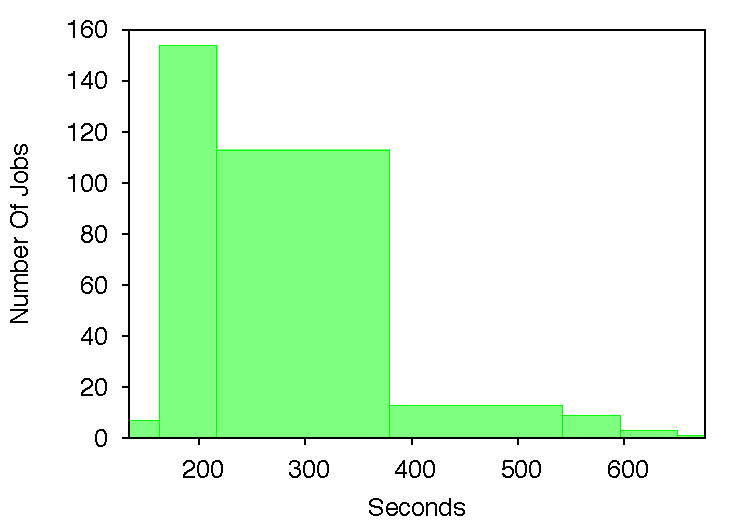
\includegraphics{images/nfs_coscheduler_tusker_histogram}
\caption{Histogram showing turnaround time distribution of 375 Jobs, when run using a coscheduler on a custom small scale independent NFS server}
\label{fig:nfs_coscheduler_tusker_histogram}
\end{center}

\begin{center}
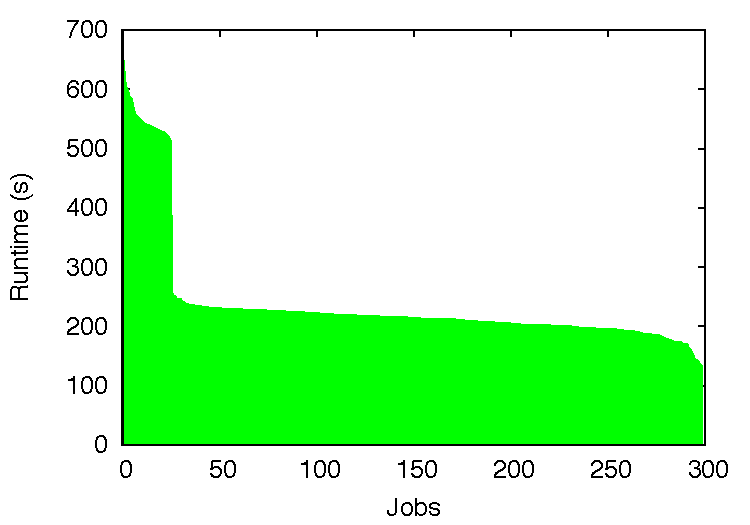
\includegraphics{images/nfs_coscheduler_tusker_goodput}
\caption{Goodput graph showing the turnaround time distribution of all the jobs submitted}
\label{fig:nfs_coscheduler_tusker_goodput}
\end{center}


\end{figure}
\FloatBarrier



In figure we can see most of the jobs take about 
500 seconds of time to complete. We've prevented excessive degradation here and 
the I/O resources serve the concurrent jobs without a degraded turnaround time. 
This reduces the total time taken for the execution of this batch of jobs 
making way for the use of cluster for other jobs that might need computing.


\begin{figure}[htbp!]
\begin{center}
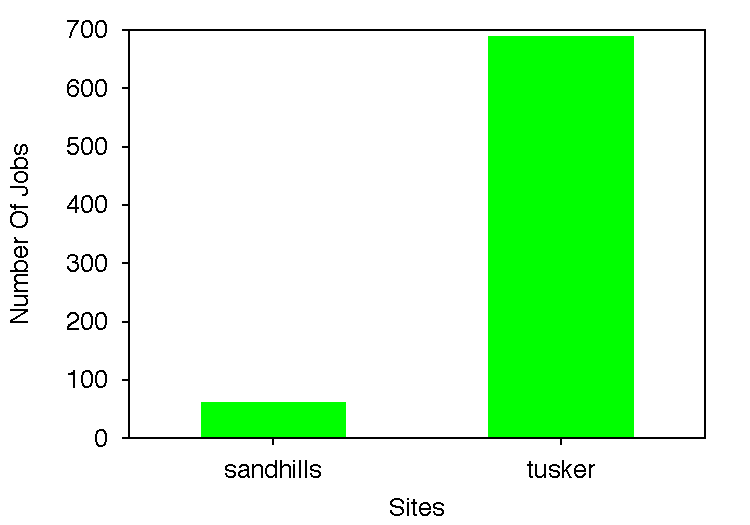
\includegraphics{images/multisite_load}
\caption{Bar plot showing load distribution}
\label{fig:multisite_load}
\end{center}
\end{figure}
\FloatBarrier


In figure \ref{fig:multisite_load}, multi-Site load distribution algorithm distributes the job based on the 
turnaround time and load on the cluster, the following was the distribution of jobs when run 
on Co-Scheduler with 750 Jobs. The cluster with lower turnaround time will get more amount of jobs to run. The average turnaround time for 
the cluster tusker is 764 seconds and the average turnaround time for the 
cluster sandhills is about 413. The lower turnaround time of sandhills is 
because of the lower availability which can be noted by the throughput information. 
For tusker the throughput was 47.2 CPU time hours/elapsed time hours and for 
sandhills it was 3.12 CPU time hours/elapsed time hours.


\chapter{Conclusion}

Co-Scheduling on the Grid is challenging with the presence of dynamically varying 
resources like Network, RAM, compute resources, all of which are available opportunistically. 
The current Co-Scheduler 
detects degradation and taxes degraded resources less in terms of scheduling 
jobs to the degraded resources. The capacity of the cluster is a varying 
quantity that determines the amount of concurrent jobs that may run without 
degradation. Co-Scheduler successfully finds the capacity of the cluster and 
maintains the capacity up-to 10 successive iterations of the scheduler before 
recalculating the capacity.

With the assumption of the availability of cluster(s)(which means further queue wait time is 
absent), the Co-Scheduler improves throughput of the job set which handles the 
case of degradation by virtue of a multi-site job distribution algorithm. Because Co-Scheduler directly effects the load on the resource, Co-Scheduler 
ensures the average overall turnaround time per job is lower.

Resource management is completely abstracted. We do not need to consider the 
allocation and management of disk I/O or RAM or Network I/O. The Co-Scheduler is 
driven by the fact that whenever a resource is overloaded it results in 
degradation and subsequently does not respond optimally or crashes. A simple and 
efficient way of tracking degradation is implemented and further monitoring the load of 
resources on the cluster. As much as this is a positive aspect of the 
Co-Scheduler, the downside is there isn't a way to tell which of the resource is 
the cause of the degradation. Because the Co-Scheduler is used with large workloads its usually known based on 
the workload the resource that is under stress.

While Co-Scheduling offers multiple enhancements for the users of large workload 
there are some of the downsides of it. Co-Scheduler submits the jobs stepwise, in 
the sense that it submits a smaller set of jobs and waits for its outcome to decide upon the quantity 
of jobs on the next iteration. This 
nature of the Co-Scheduler can accumulate lot of queue wait time if the availability 
of the compute resources are lower. In the multi-site load distribution 
algorithm if one of the sites has very low availability the Co-Scheduler would 
accumulate the queue wait time of that particular site before it can complete 
its execution. The pre-emption of jobs and rescheduling to enhance such 
behavior is thus part of the future work.

%% backmatter is needed at the end of the main body of your thesis to
%% set up page numbering correctly for the remainder of the thesis
\backmatter

%% Start the correct formatting for the appendices
\appendix

%% Appendices go here (if you have them)

%% Bibliography goes here (You better have one)
%% BibTeX is your friend
%% Index go here (if you have one)
%% Bibliography goes here (You better have one)
%% BibTeX is your friend
\bibliographystyle{plain}
\bibliography{KartikThesis}
%% Pull in all the entries in the bibtex file. Is is a useful trick to
%% check all your references.
\nocite{*}

%% Index go here (if you have one)

\end{document}